\documentclass[14pt]{extbook}
\usepackage{multicol, enumerate, enumitem, hyperref, color, soul, setspace, parskip, fancyhdr} %General Packages
\usepackage{amssymb, amsthm, amsmath, bbm, latexsym, units, mathtools} %Math Packages
\everymath{\displaystyle} %All math in Display Style
% Packages with additional options
\usepackage[headsep=0.5cm,headheight=12pt, left=1 in,right= 1 in,top= 1 in,bottom= 1 in]{geometry}
\usepackage[usenames,dvipsnames]{xcolor}
\usepackage{dashrule}  % Package to use the command below to create lines between items
\newcommand{\litem}[1]{\item#1\hspace*{-1cm}\rule{\textwidth}{0.4pt}}
\pagestyle{fancy}
\lhead{Progress Quiz 9}
\chead{}
\rhead{Version A}
\lfoot{8590-6105}
\cfoot{}
\rfoot{Fall 2020}
\begin{document}

\begin{enumerate}
\litem{
Determine the vertical asymptotes and holes in the rational function below.\[ f(x) = \frac{12x^{3} +23 x^{2} -8 x -12}{9x^{2} -9 x -10} \]\begin{enumerate}[label=\Alph*.]
\item \( \text{Holes at } x = 1.667 \text{ and } x = -0.667 \text{ with no vertical asymptotes.} \)
\item \( \text{Vertical Asymptotes of } x = 1.667 \text{ and } x = 0.75 \text{ with a hole at } x = -0.667 \)
\item \( \text{Vertical Asymptote of } x = 1.667 \text{ and hole at } x = -0.667 \)
\item \( \text{Vertical Asymptote of } x = 1.333 \text{ and hole at } x = -0.667 \)
\item \( \text{Vertical Asymptotes of } x = 1.667 \text{ and } x = -0.667 \text{ with no holes.} \)

\end{enumerate} }
\litem{
Determine the horizontal and/or oblique asymptotes in the rational function below.\[ f(x) = \frac{2x^{2} -x -6}{10x^{3} +33 x^{2} +35 x + 12} \]\begin{enumerate}[label=\Alph*.]
\item \( \text{Horizontal Asymptote at } y = 2.000 \)
\item \( \text{Horizontal Asymptote of } y = 0 \)
\item \( \text{Horizontal Asymptote of } y = 0.200 \text{ and Oblique Asymptote of } y = 5x + 19 \)
\item \( \text{Horizontal Asymptote of } y = 0.200  \)
\item \( \text{Oblique Asymptote of } y = 5x + 19. \)

\end{enumerate} }
\litem{
Determine the horizontal and/or oblique asymptotes in the rational function below.\[ f(x) = \frac{6x^{3} +13 x^{2} -13 x -30}{2x^{2} -9 x + 9} \]\begin{enumerate}[label=\Alph*.]
\item \( \text{Horizontal Asymptote of } y = 3.0  \)
\item \( \text{Horizontal Asymptote of } y = 3.0 \text{ and Oblique Asymptote of } y = 3x + 20 \)
\item \( \text{Horizontal Asymptote of } y = 3.0 \text{ and Oblique Asymptote of } y = 3x + 20 \)
\item \( \text{Horizontal Asymptote at } y = 3.0 \)
\item \( \text{Oblique Asymptote of } y = 3x + 20. \)

\end{enumerate} }
\litem{
Determine the vertical asymptotes and holes in the rational function below.\[ f(x) = \frac{12x^{3} +71 x^{2} +102 x + 40}{8x^{2} -2 x -15} \]\begin{enumerate}[label=\Alph*.]
\item \( \text{Vertical Asymptote of } x = 1.5 \text{ and hole at } x = -1.25 \)
\item \( \text{Holes at } x = 1.5 \text{ and } x = -1.25 \text{ with no vertical asymptotes.} \)
\item \( \text{Vertical Asymptotes of } x = 1.5 \text{ and } x = -1.25 \text{ with no holes.} \)
\item \( \text{Vertical Asymptote of } x = 1.5 \text{ and hole at } x = -1.25 \)
\item \( \text{Vertical Asymptotes of } x = 1.5 \text{ and } x = -0.667 \text{ with a hole at } x = -1.25 \)

\end{enumerate} }
\litem{
Which of the following functions \textit{could} be the graph below?
\begin{center}
    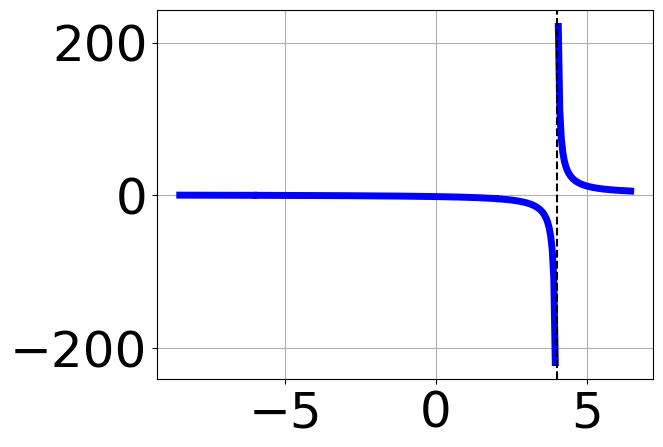
\includegraphics[width=0.5\textwidth]{../Figures/identifyGraphOfRationalFunctionA.png}
\end{center}
\begin{enumerate}[label=\Alph*.]
\item \( f(x)=\frac{x^{3} +11 x^{2} +16 x -84}{x^{3} -28 x + 48} \)
\item \( f(x)=\frac{x^{3} -11 x^{2} +16 x + 84}{x^{3} -28 x -48} \)
\item \( f(x)=\frac{x^{3} -11 x^{2} +16 x + 84}{x^{3} -28 x -48} \)
\item \( f(x)=\frac{x^{3} +10 x^{2} +17 x -28}{x^{3} -28 x + 48} \)
\item \( \text{None of the above are possible equations for the graph.} \)

\end{enumerate} }
\litem{
Determine the vertical asymptotes and holes in the rational function below.\[ f(x) = \frac{12x^{3} -13 x^{2} -5 x + 6}{9x^{2} -6 x -8} \]\begin{enumerate}[label=\Alph*.]
\item \( \text{Vertical Asymptotes of } x = 1.333 \text{ and } x = 0.75 \text{ with a hole at } x = -0.667 \)
\item \( \text{Vertical Asymptote of } x = 1.333 \text{ and hole at } x = -0.667 \)
\item \( \text{Vertical Asymptote of } x = 1.333 \text{ and hole at } x = -0.667 \)
\item \( \text{Holes at } x = 1.333 \text{ and } x = -0.667 \text{ with no vertical asymptotes.} \)
\item \( \text{Vertical Asymptotes of } x = 1.333 \text{ and } x = -0.667 \text{ with no holes.} \)

\end{enumerate} }
\litem{
Determine the horizontal and/or oblique asymptotes in the rational function below.\[ f(x) = \frac{8x^{3} -6 x^{2} -65 x + 75}{4x^{3} +6 x^{2} +13 x -60} \]\begin{enumerate}[label=\Alph*.]
\item \( \text{Vertical Asymptote of } y = -3  \)
\item \( \text{Vertical Asymptote of } y = -4.000  \)
\item \( \text{Horizontal Asymptote of } y = 2.000  \)
\item \( \text{None of the above} \)
\item \( \text{Horizontal Asymptote of } y = 0  \)

\end{enumerate} }
\litem{
Determine the horizontal and/or oblique asymptotes in the rational function below.\[ f(x) = \frac{9x^{3} -30 x^{2} -11 x + 60}{3x^{2} -5 x -12} \]\begin{enumerate}[label=\Alph*.]
\item \( \text{Oblique Asymptote of } y = 3x -5. \)
\item \( \text{Horizontal Asymptote of } y = 3.0  \)
\item \( \text{Horizontal Asymptote of } y = 3.0 \text{ and Oblique Asymptote of } y = 3x -5 \)
\item \( \text{Horizontal Asymptote of } y = 3.0 \text{ and Oblique Asymptote of } y = 3x -5 \)
\item \( \text{Horizontal Asymptote at } y = 3.0 \)

\end{enumerate} }
\litem{
Determine the vertical asymptotes and holes in the rational function below.\[ f(x) = \frac{9x^{3} -27 x^{2} -4 x + 12}{9x^{2} -9 x -10} \]\begin{enumerate}[label=\Alph*.]
\item \( \text{Vertical Asymptotes of } x = 1.667 \text{ and } x = -0.667 \text{ with no holes.} \)
\item \( \text{Vertical Asymptote of } x = 1.0 \text{ and hole at } x = -0.667 \)
\item \( \text{Vertical Asymptote of } x = 1.667 \text{ and hole at } x = -0.667 \)
\item \( \text{Vertical Asymptotes of } x = 1.667 \text{ and } x = 0.667 \text{ with a hole at } x = -0.667 \)
\item \( \text{Holes at } x = 1.667 \text{ and } x = -0.667 \text{ with no vertical asymptotes.} \)

\end{enumerate} }
\litem{
Which of the following functions \textit{could} be the graph below?
\begin{center}
    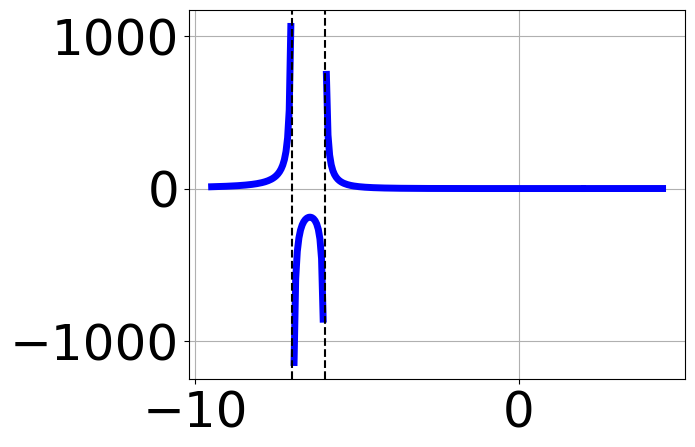
\includegraphics[width=0.5\textwidth]{../Figures/identifyGraphOfRationalFunctionCopyA.png}
\end{center}
\begin{enumerate}[label=\Alph*.]
\item \( f(x)=\frac{x^{3} +4 x^{2} -4 x -16}{x^{3} -11 x^{2} +16 x + 84} \)
\item \( f(x)=\frac{x^{3} -4 x^{2} -4 x + 16}{x^{3} +11 x^{2} +16 x -84} \)
\item \( f(x)=\frac{x^{3} +2 x^{2} -16 x -32}{x^{3} +11 x^{2} +16 x -84} \)
\item \( f(x)=\frac{x^{3} +4 x^{2} -4 x -16}{x^{3} -11 x^{2} +16 x + 84} \)
\item \( \text{None of the above are possible equations for the graph.} \)

\end{enumerate} }
\end{enumerate}

\end{document}